\chapter{Interpretation}
\label{chap:interp}

Since no events are observed, limits are set on the parameter space of \ac{GMSB} \ac{SUSY} mdoels. Limits are computed using HistFitter \cite{histfitter}, an \ac{ATLAS} framework that combines the observed number of events with uncertainties on background predictions and signal systematics and calculates both model dependent and model independent limits using the CL$_{\text{s}}$ technique \cite{CLs-1}. CL$_{\text{s}}$ is a useful tool for particle physics analyses. Somewhere between a purely frequentist and purlely basian method of deriving a confidence interval, the CL$_{\text{s}}$ describes the confidence in a signal-only hypothesis. The limit curve is drawn where CL$_{\text{s}}(m_{\tilde{\ell}}) \leq 5\%$, meaning that the probability of having falsely excluded a \slep of a given mass is less than or equal to 5\%. The smaller the value of CL$_{\text{s}}$, the lower the probability that a \slep with a given mass exists. For a search where 0 background events are predicted, 3 events are required for a 95\% CL$_{\text{s}}$~\cite{better-than-zero}.

\section{Slepton Limits}
Limits are set on the possible masses and lifetimes of long-lived \slep. Four different limits are set using the results of this analysis: each \selec, \smu, or \stau \ac{NLSP}, or the mass degenerate case with all three as co-\ac{NLSP}s. Results for all four scenarios combined are shown in \autoref{fig:excl_limit}, and the individual limit for each of the four scenarios along with their observed CL$_{\text{s}}$ value is shown in \autoref{fig:plot_cls}.

For the \selec \ac{NLSP} and \smu \ac{NLSP} cases, the results from SR-$ee$ and SR-$\mu\mu$, respectively, are used. While for the \stau and co-\ac{NLSP} cases, all three SRs are combined. For a lifetime of 0.1 ns, \selec NLSP, \smu \ac{NLSP}, \stau \ac{NLSP}, and co-NLSP scenarios are excluded for \slep masses up to 720~\GeV, 680~\GeV, 340~\GeV, and 820~\GeV, respectively. Co-NSLP events are also excluded up to 10 ns for masses below 330~\GeV. The previous from OPAL~\cite{opal} is surpassed by nearly an order of magnitude for \selec-, \smu-, and co-NSLP scenarios.


 \begin{figure}[!ht]
    \centering
        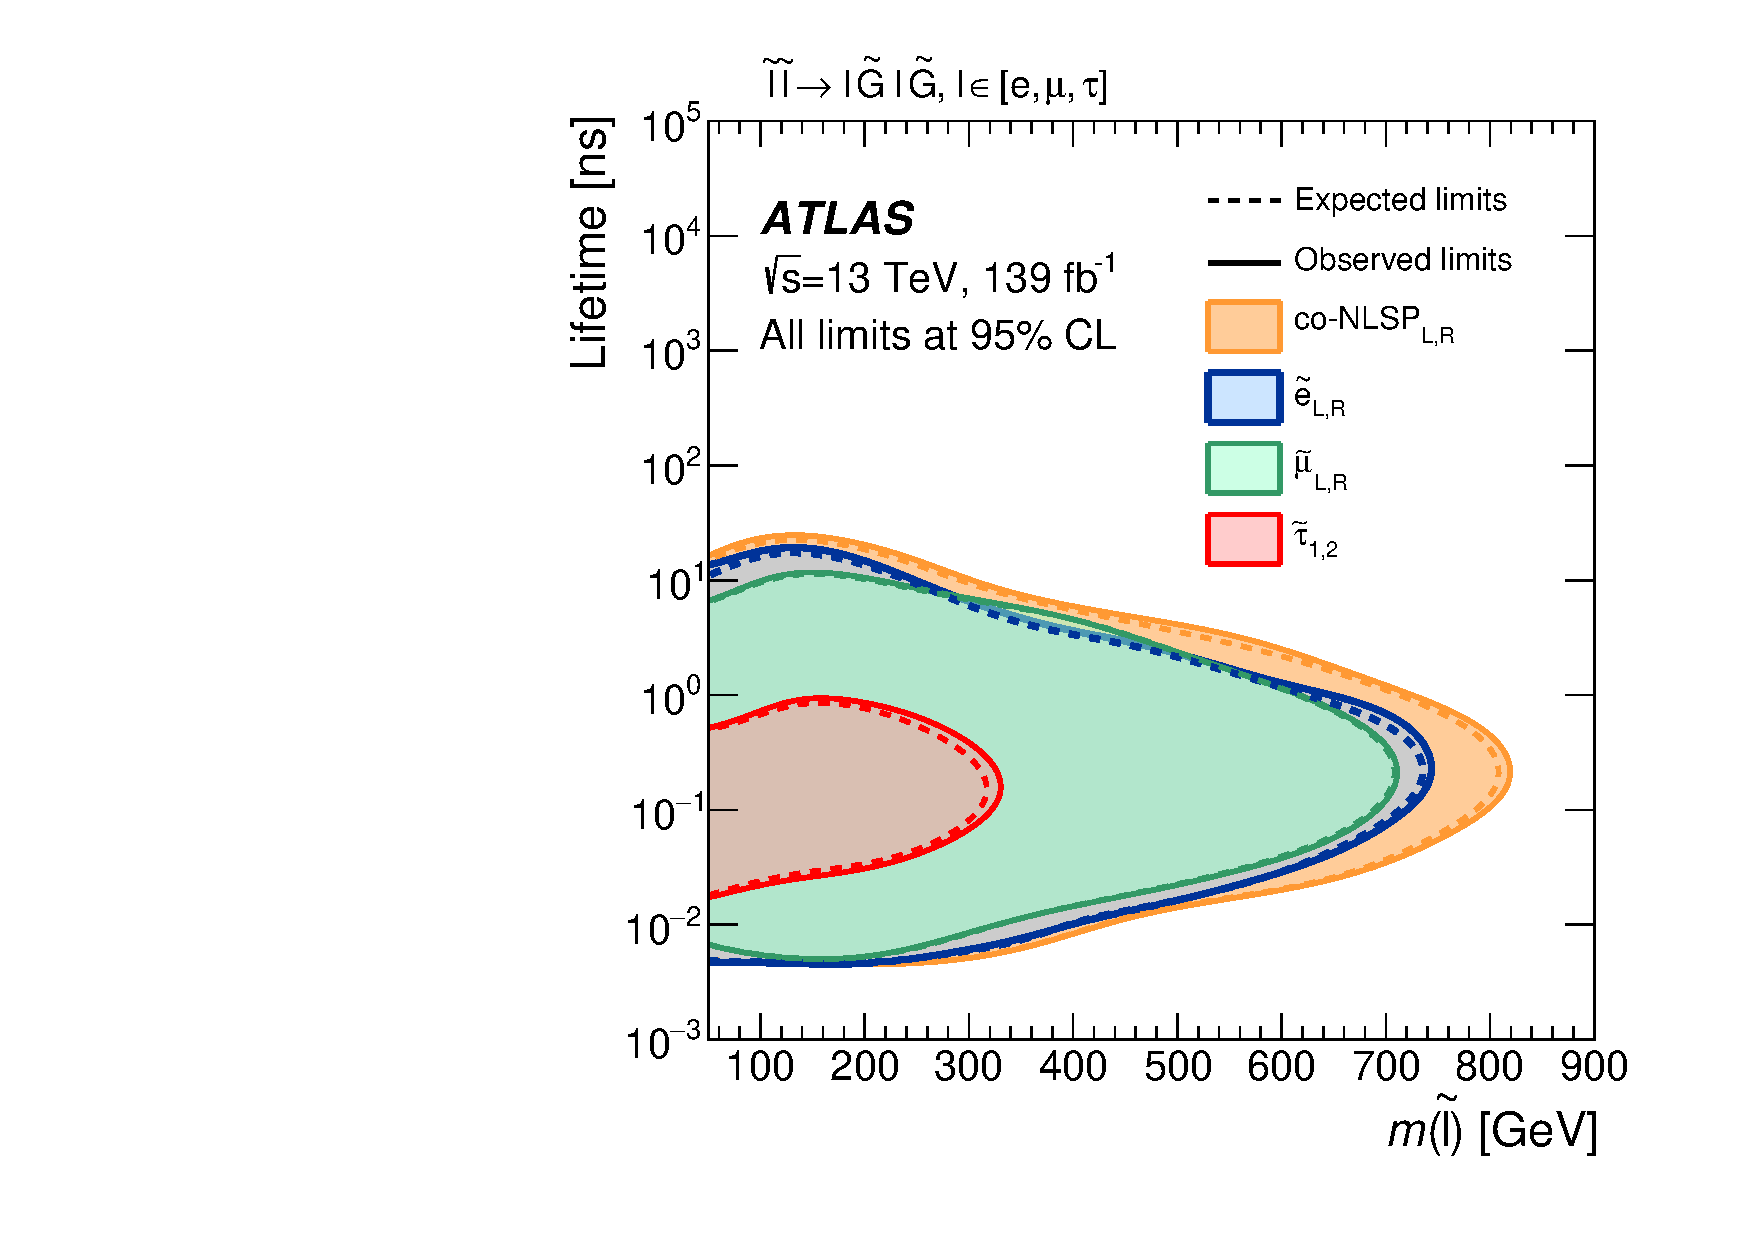
\includegraphics[width=0.6\textwidth]{figures/limits/displaced_lepton_summary.pdf}
    \caption{
    Expected (dashed) and observed (solid) exclusion contours for $\tilde{e}$ \ac{NLSP}, $\tilde{\mu}$ \ac{NLSP}, $\tilde{\tau}$ \ac{NLSP}, and co-NLSP production as a function of the lifetime at 95\% CL.
    }
    \label{fig:excl_limit}
\end{figure}

\begin{figure}[!ht]
    \centering
        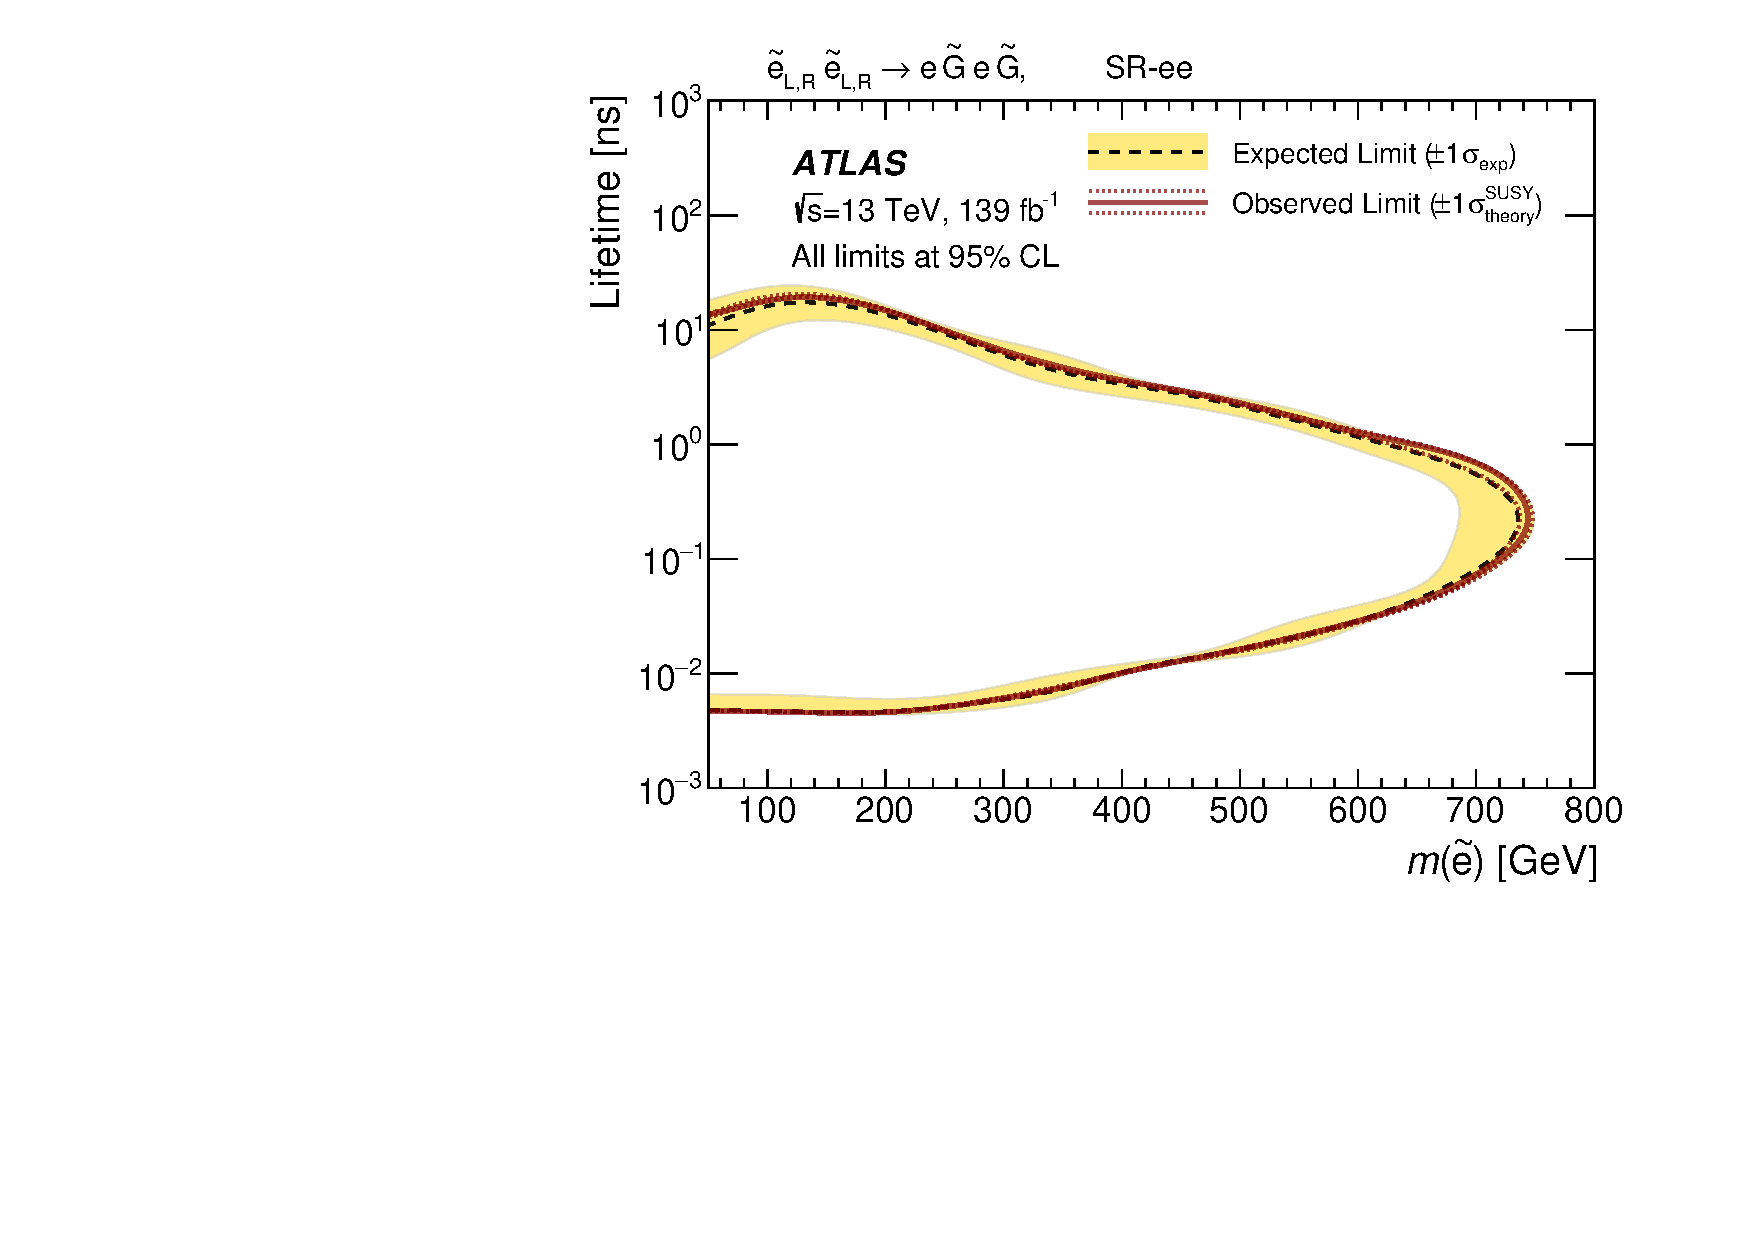
\includegraphics[width=0.45\textwidth]{figures/limits/SRee_Slep.pdf}
        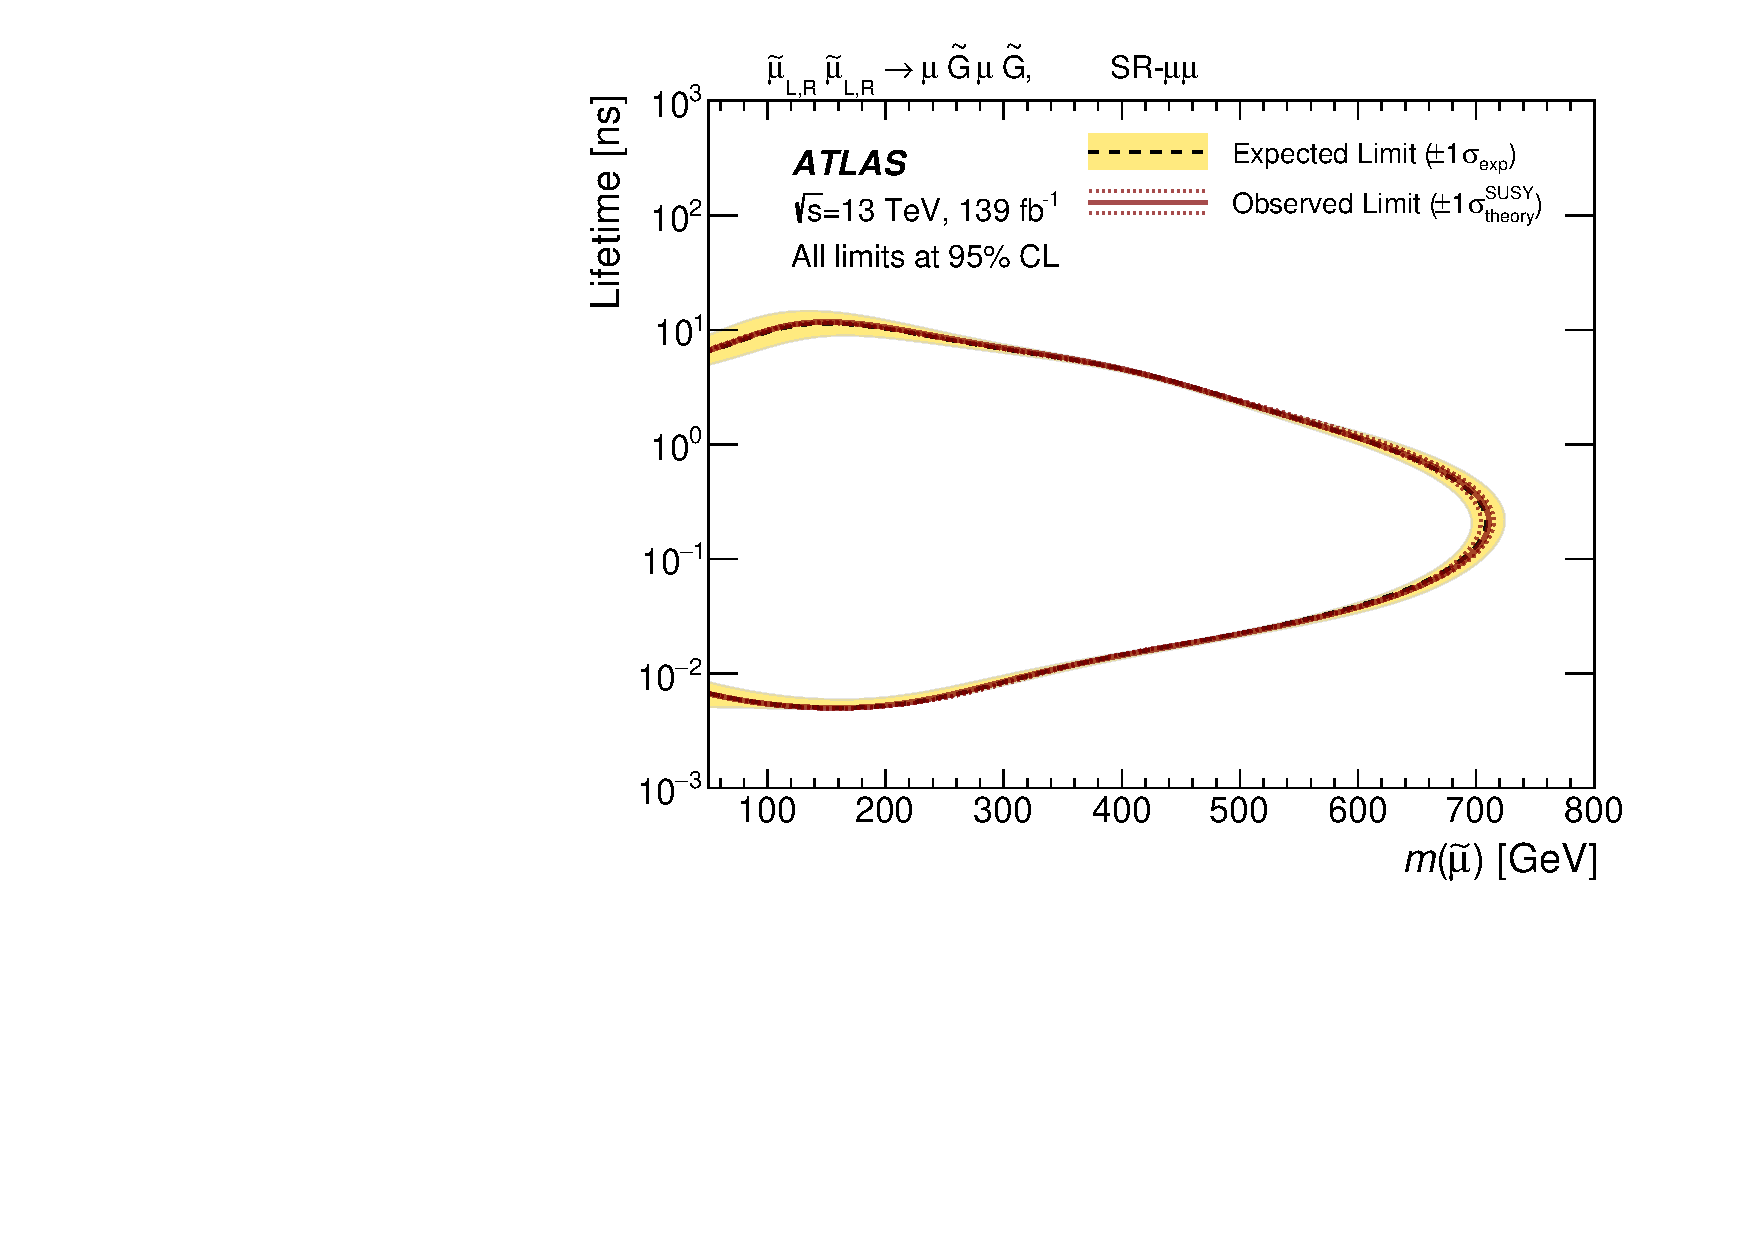
\includegraphics[width=0.45\textwidth]{figures/limits/SRmm_Slep.pdf}
        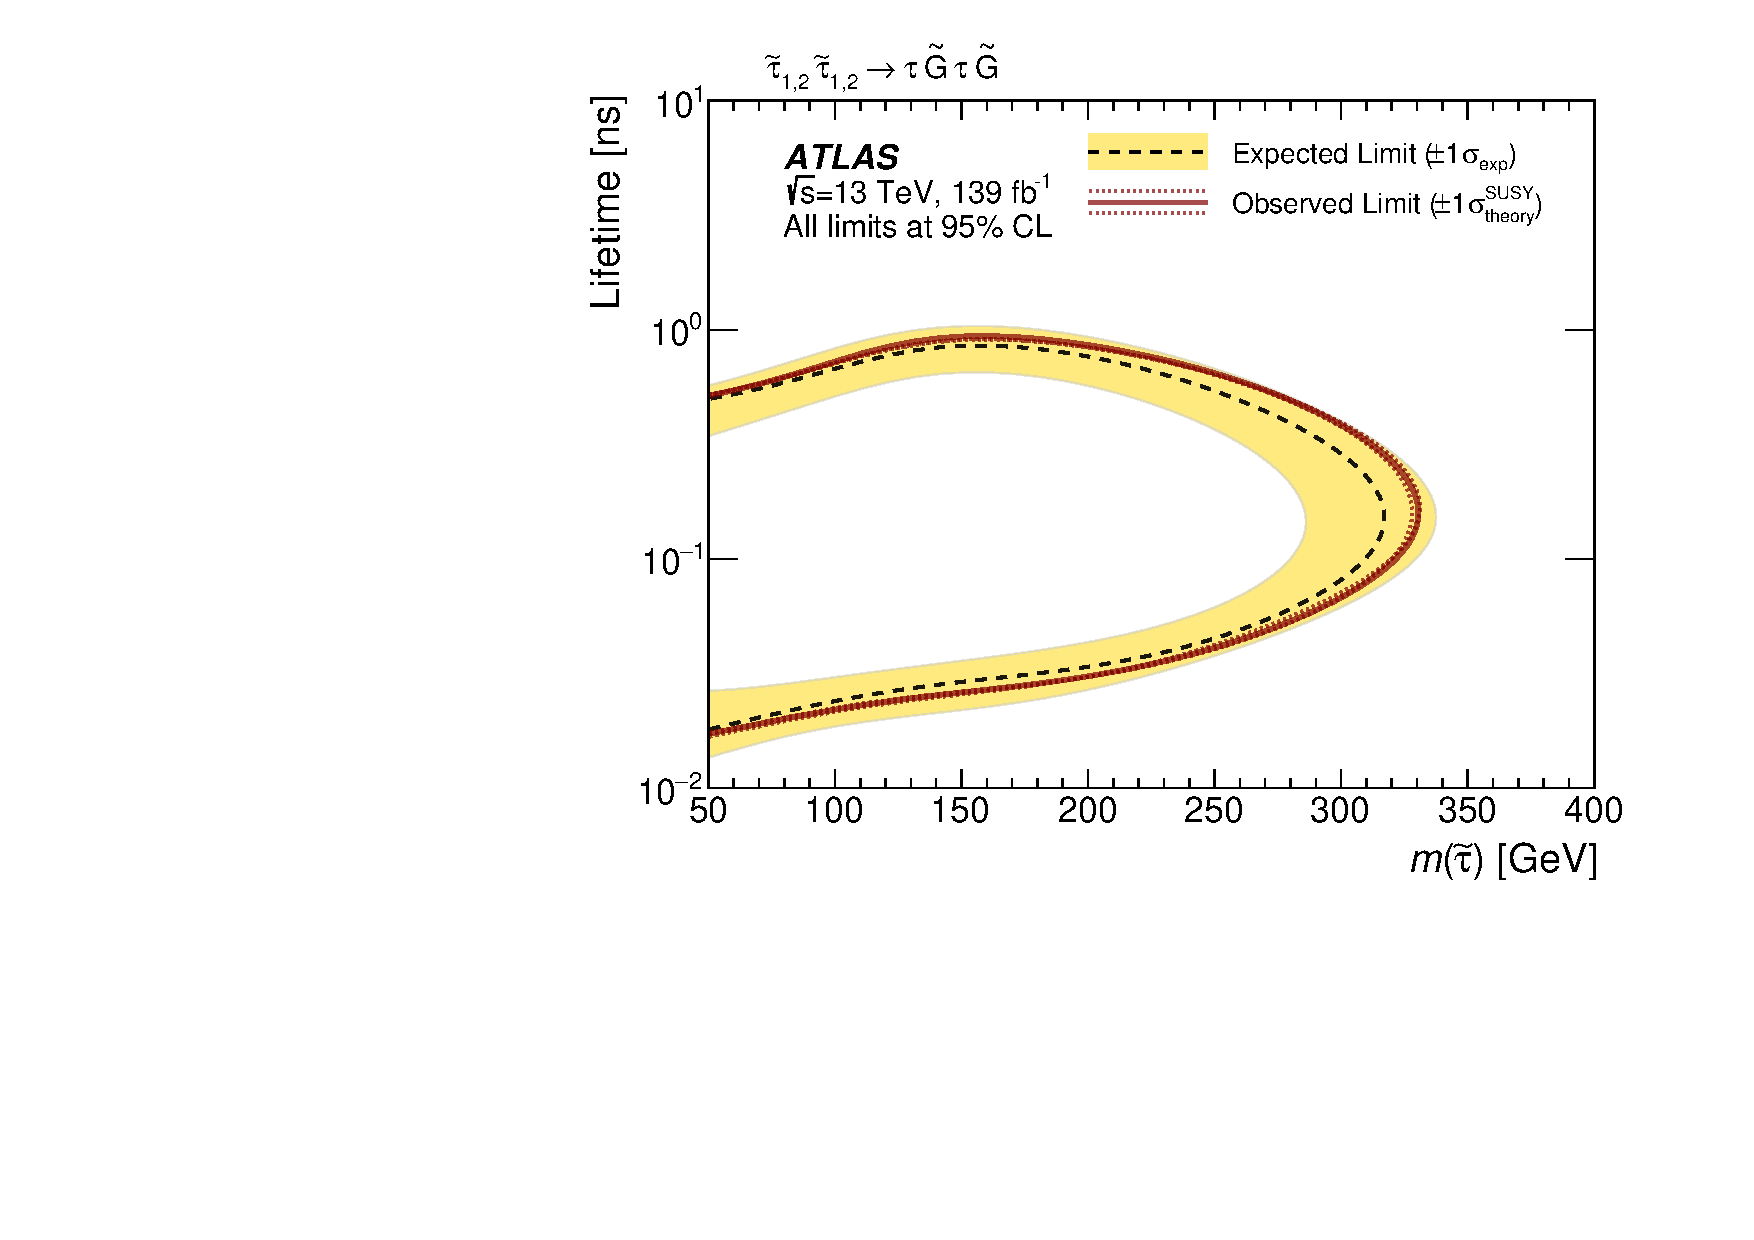
\includegraphics[width=0.45\textwidth]{figures/limits/Stau.pdf}
        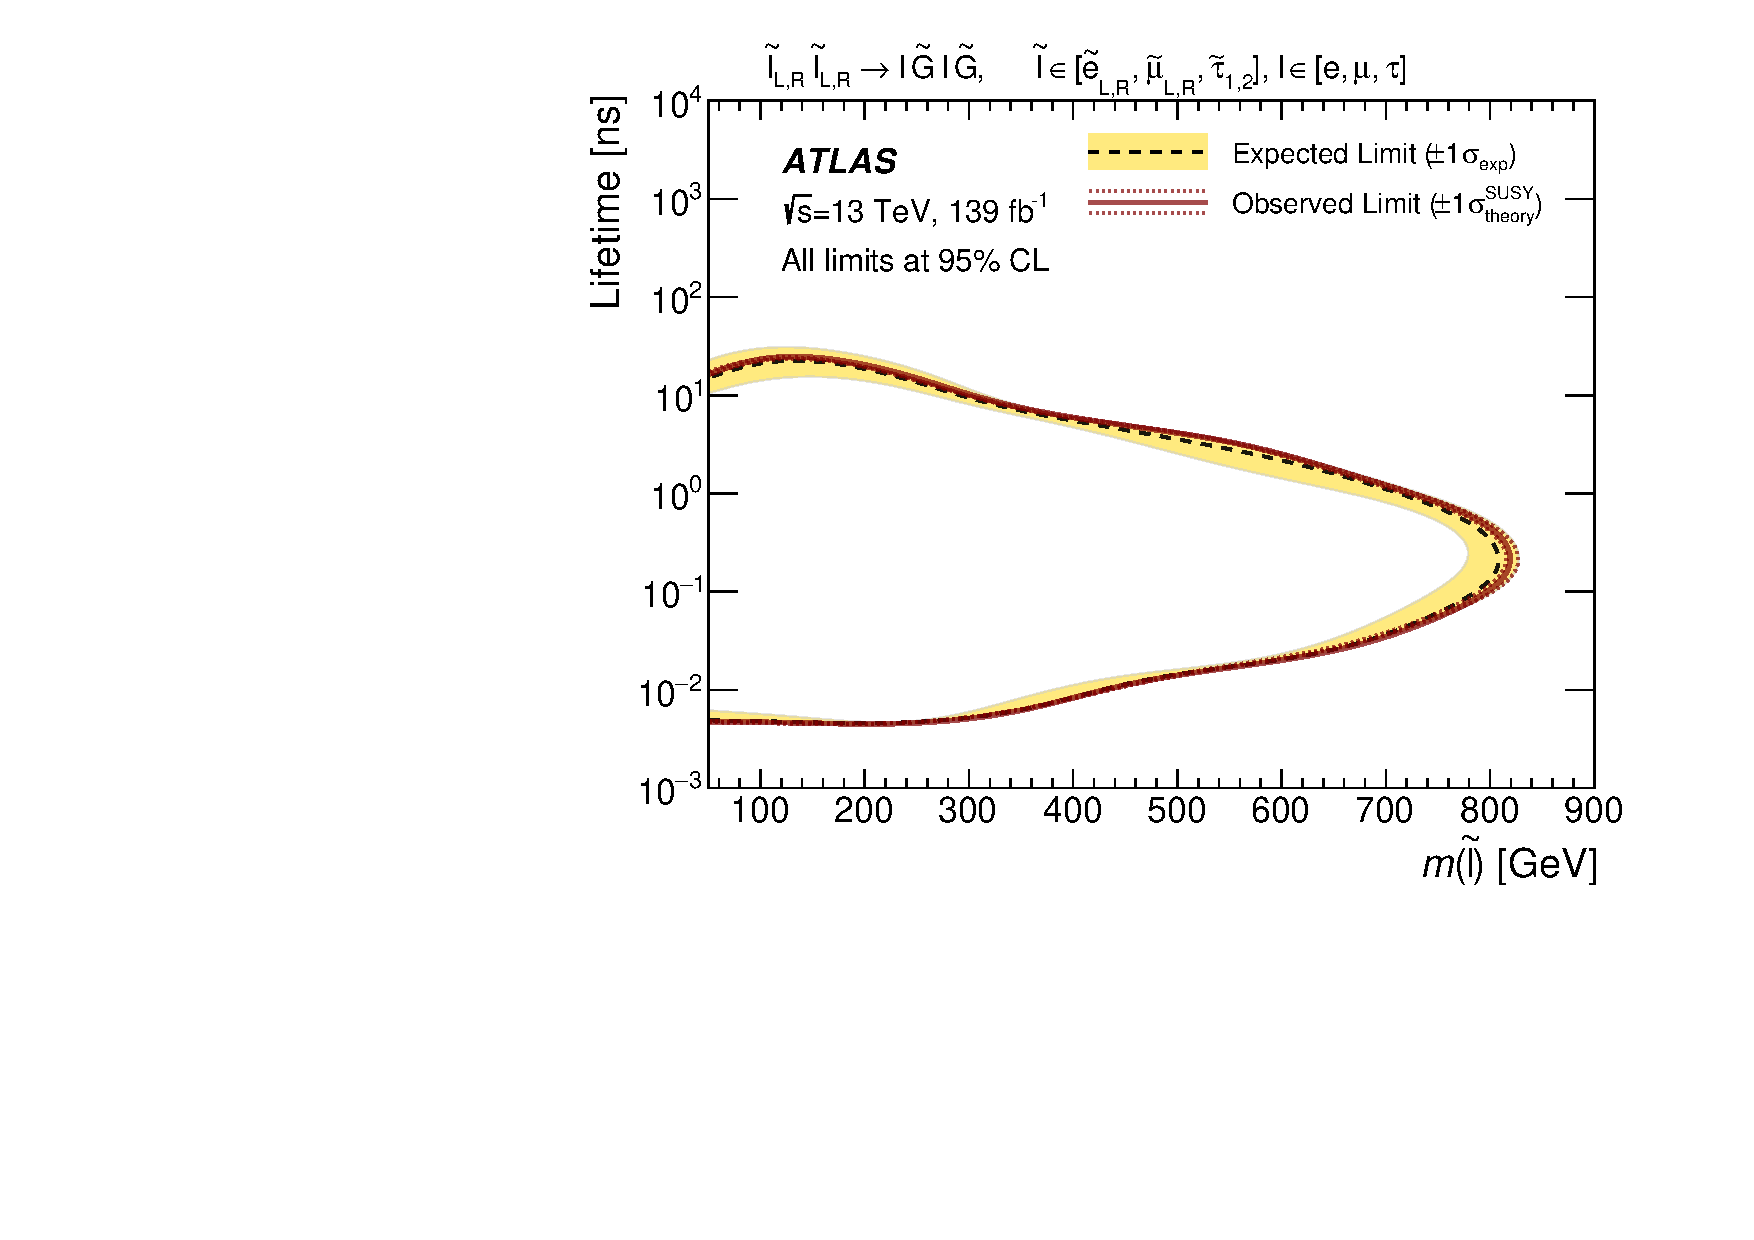
\includegraphics[width=0.45\textwidth]{figures/limits/Comb.pdf}
    \caption{Individual exclusion curves for four different \ac{NLSP} scenarios: \selec (top left), \smu (top right), \stau (bottom left), co-\ac{NLSP} (bottom right).}
    \label{fig:plot_cls}
\end{figure}

\subsection{Comparison to LEP}

The summary in \autoref{fig:excl_limit} includes both right- and left-handed slepton production and cannot be directly compared to the results from \ac{LEP}. Right-handed only or left-handed only, as well as $\stau_1$ and $\stau_2$ limits are shown in \autoref{fig:lep_comp} and compared to the LEP limit where possible.

\begin{figure}[!ht]
    \centering
        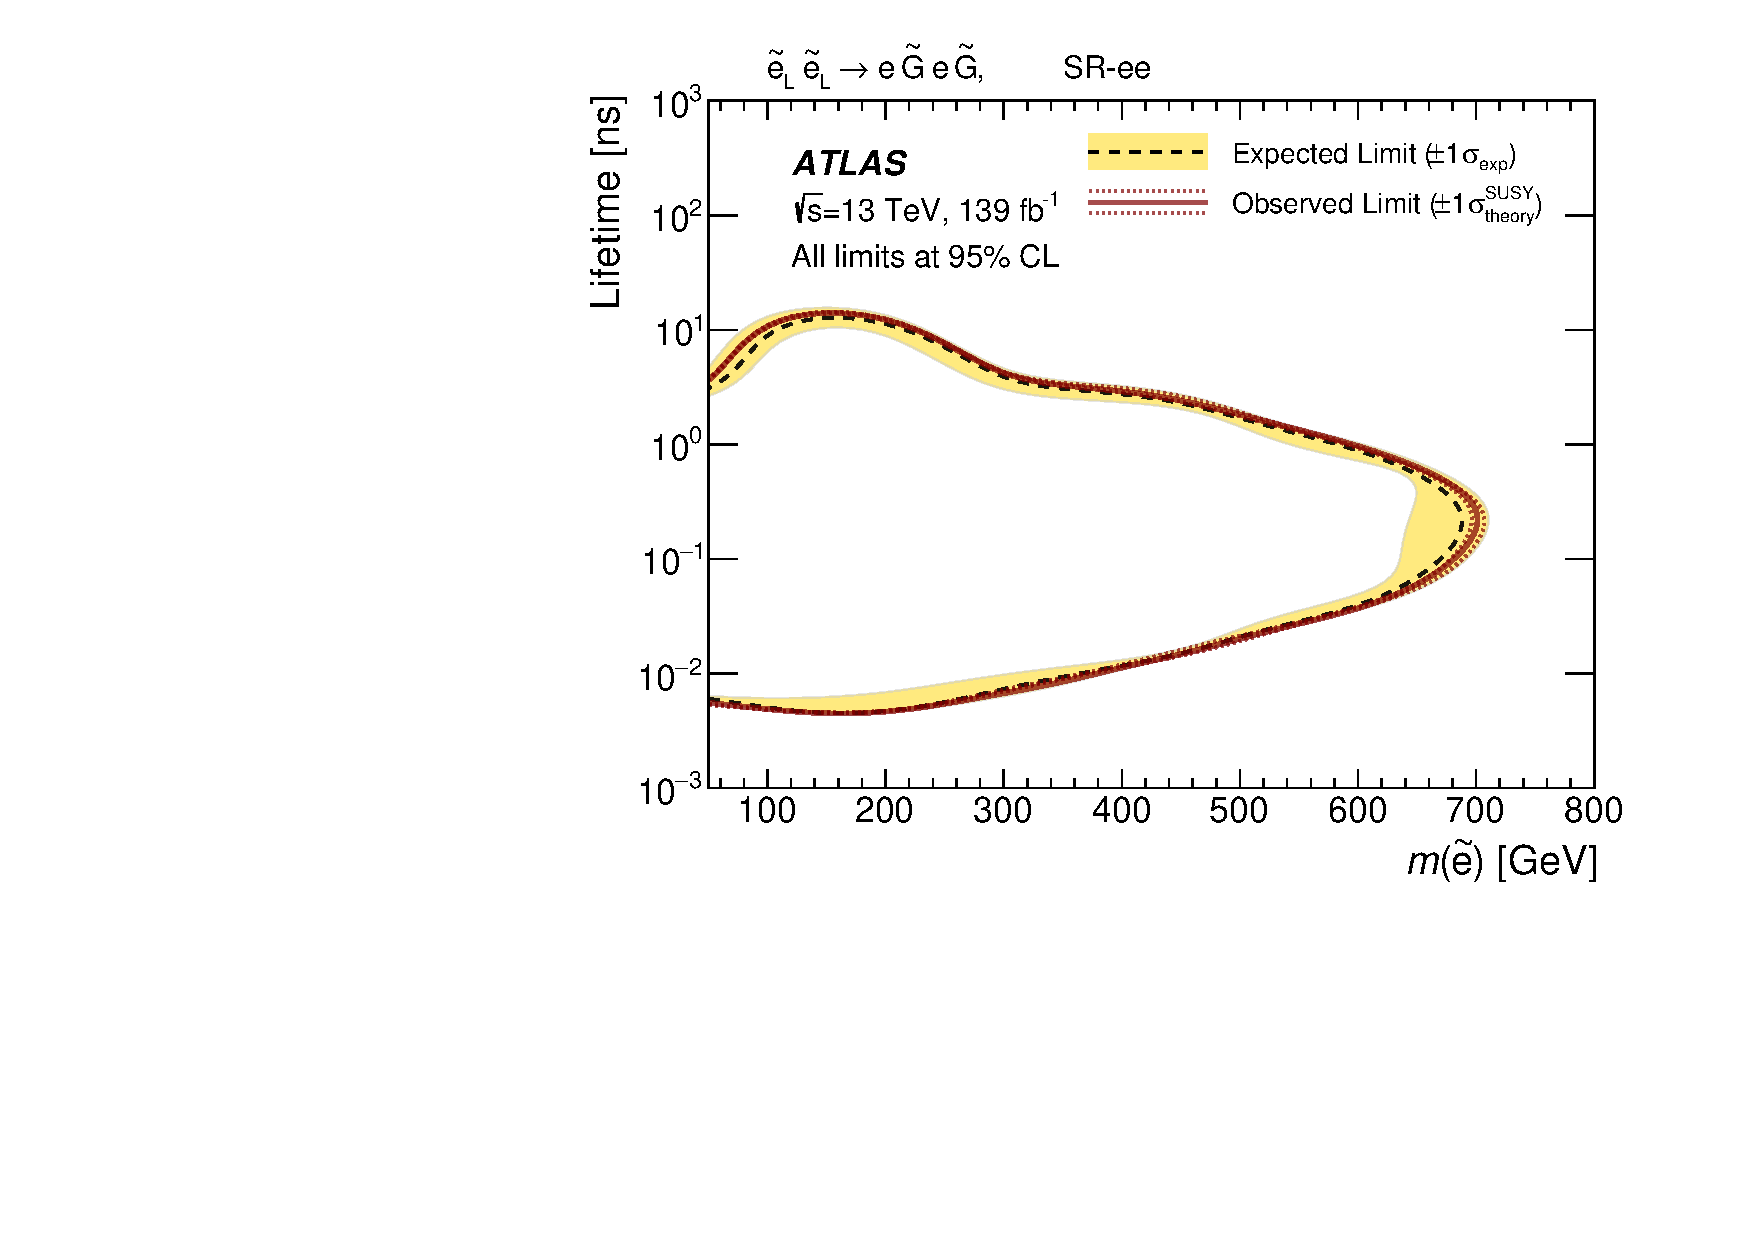
\includegraphics[width=0.45\textwidth]{figures/limits/SRee_Slepleft.pdf}
        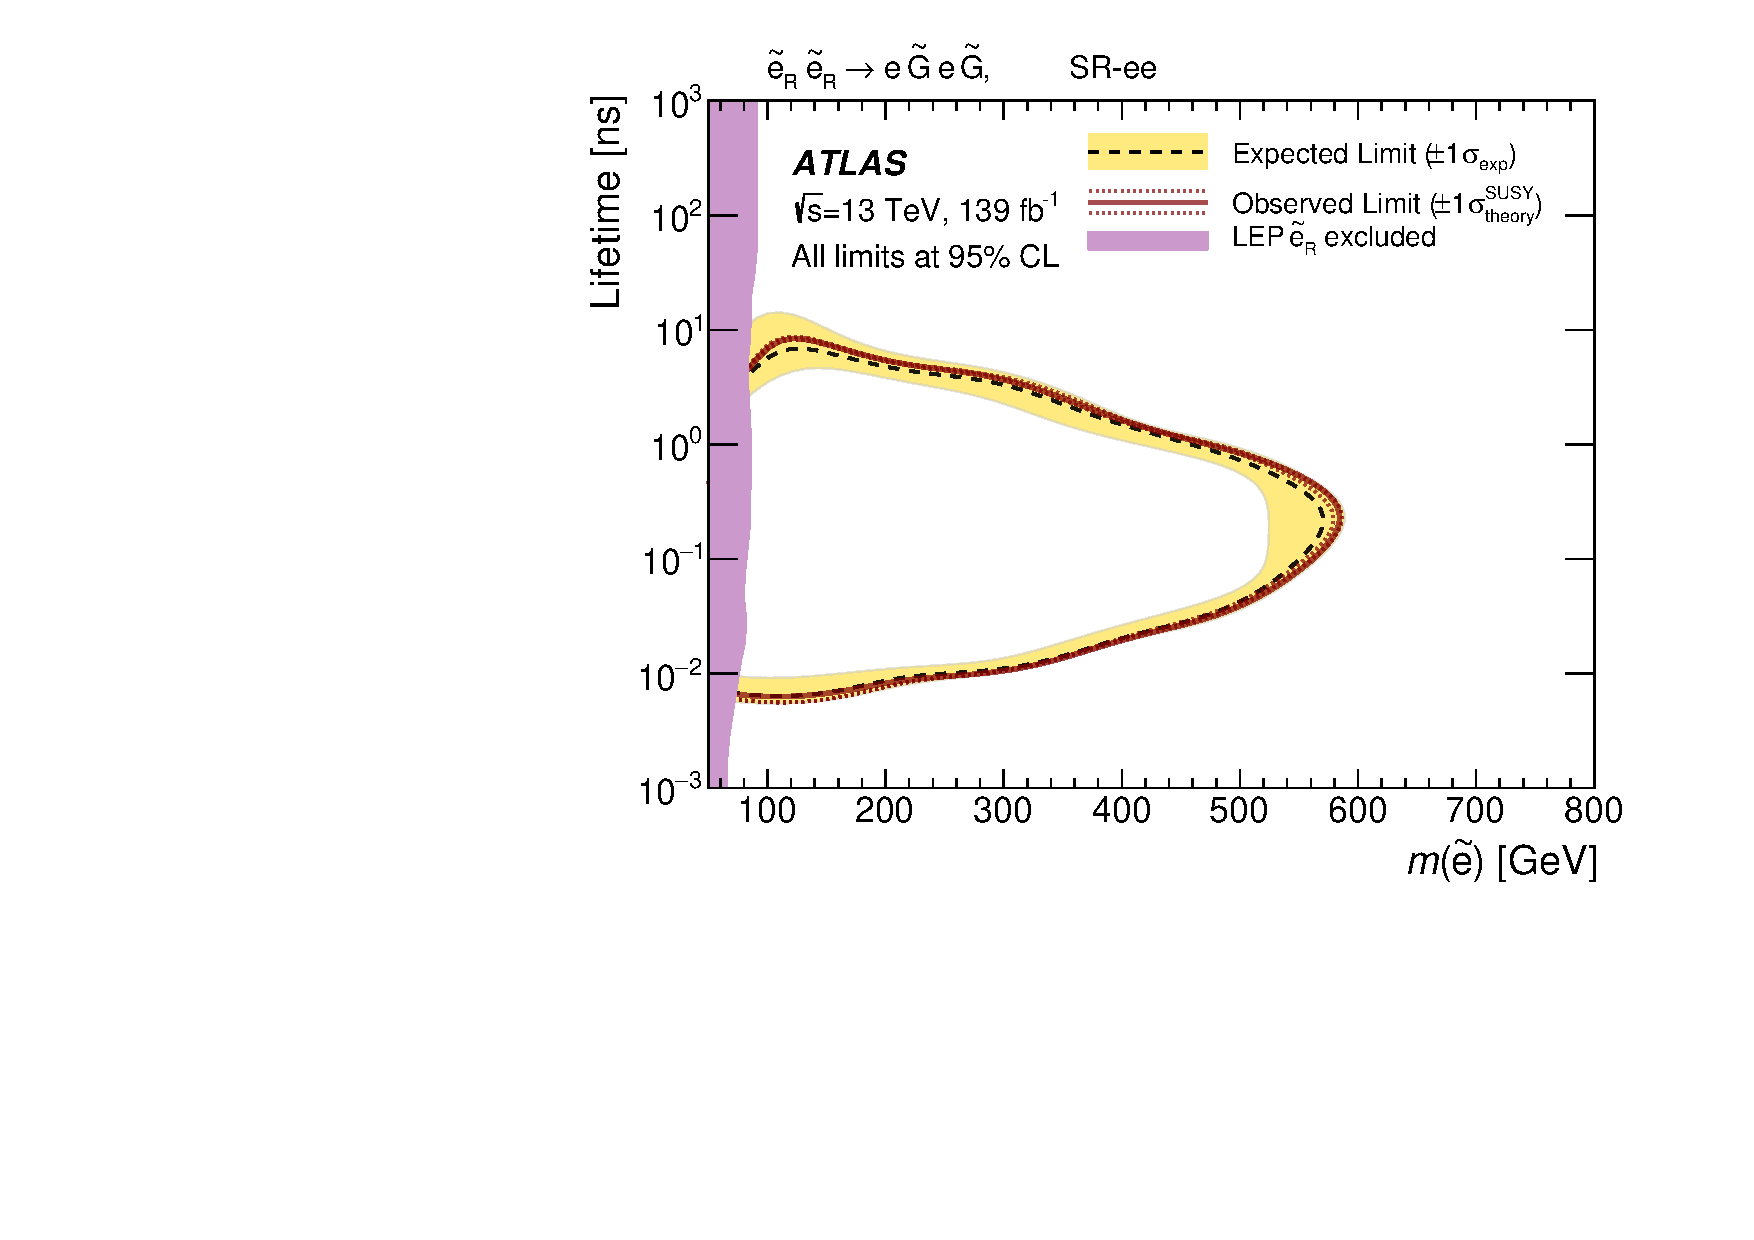
\includegraphics[width=0.45\textwidth]{figures/limits/SRee_Slepright.pdf}
        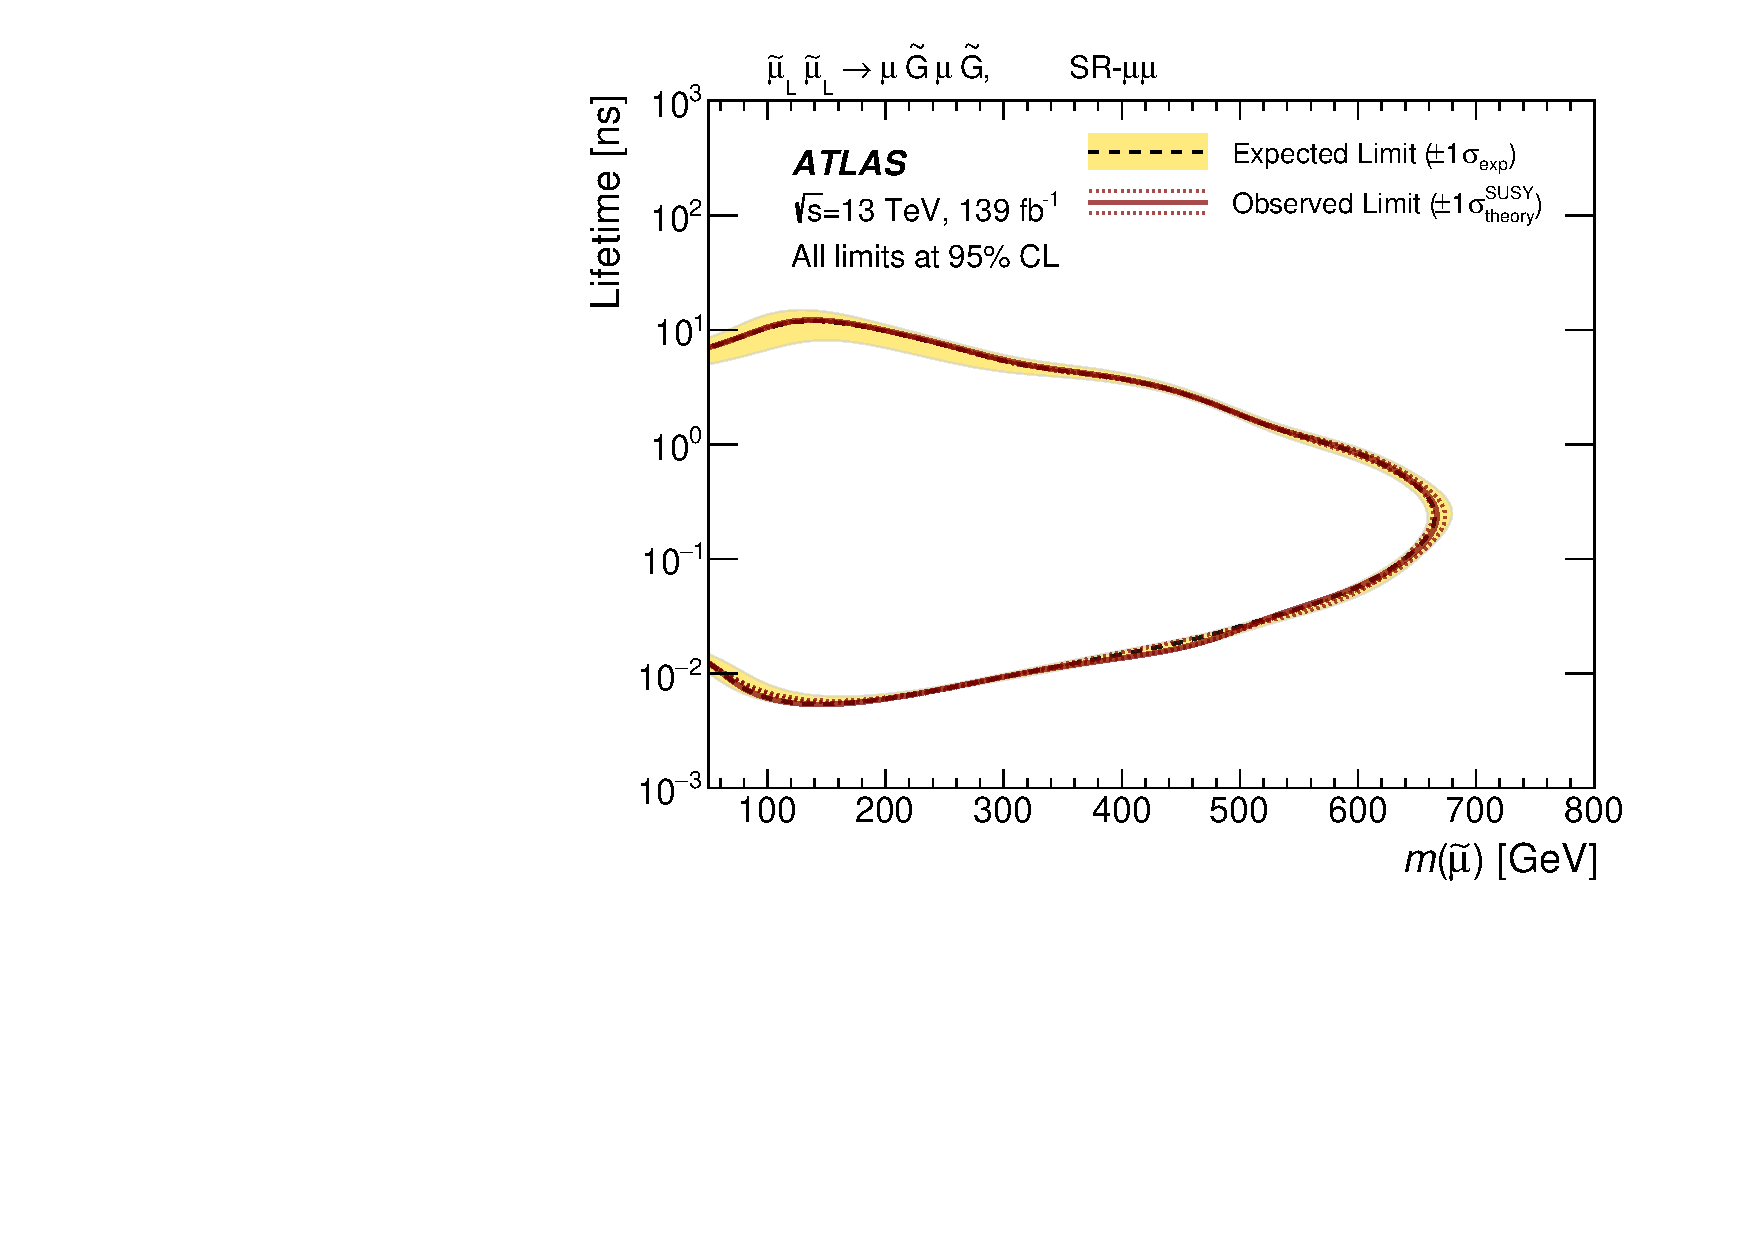
\includegraphics[width=0.45\textwidth]{figures/limits/SRmm_Slepleft.pdf}
        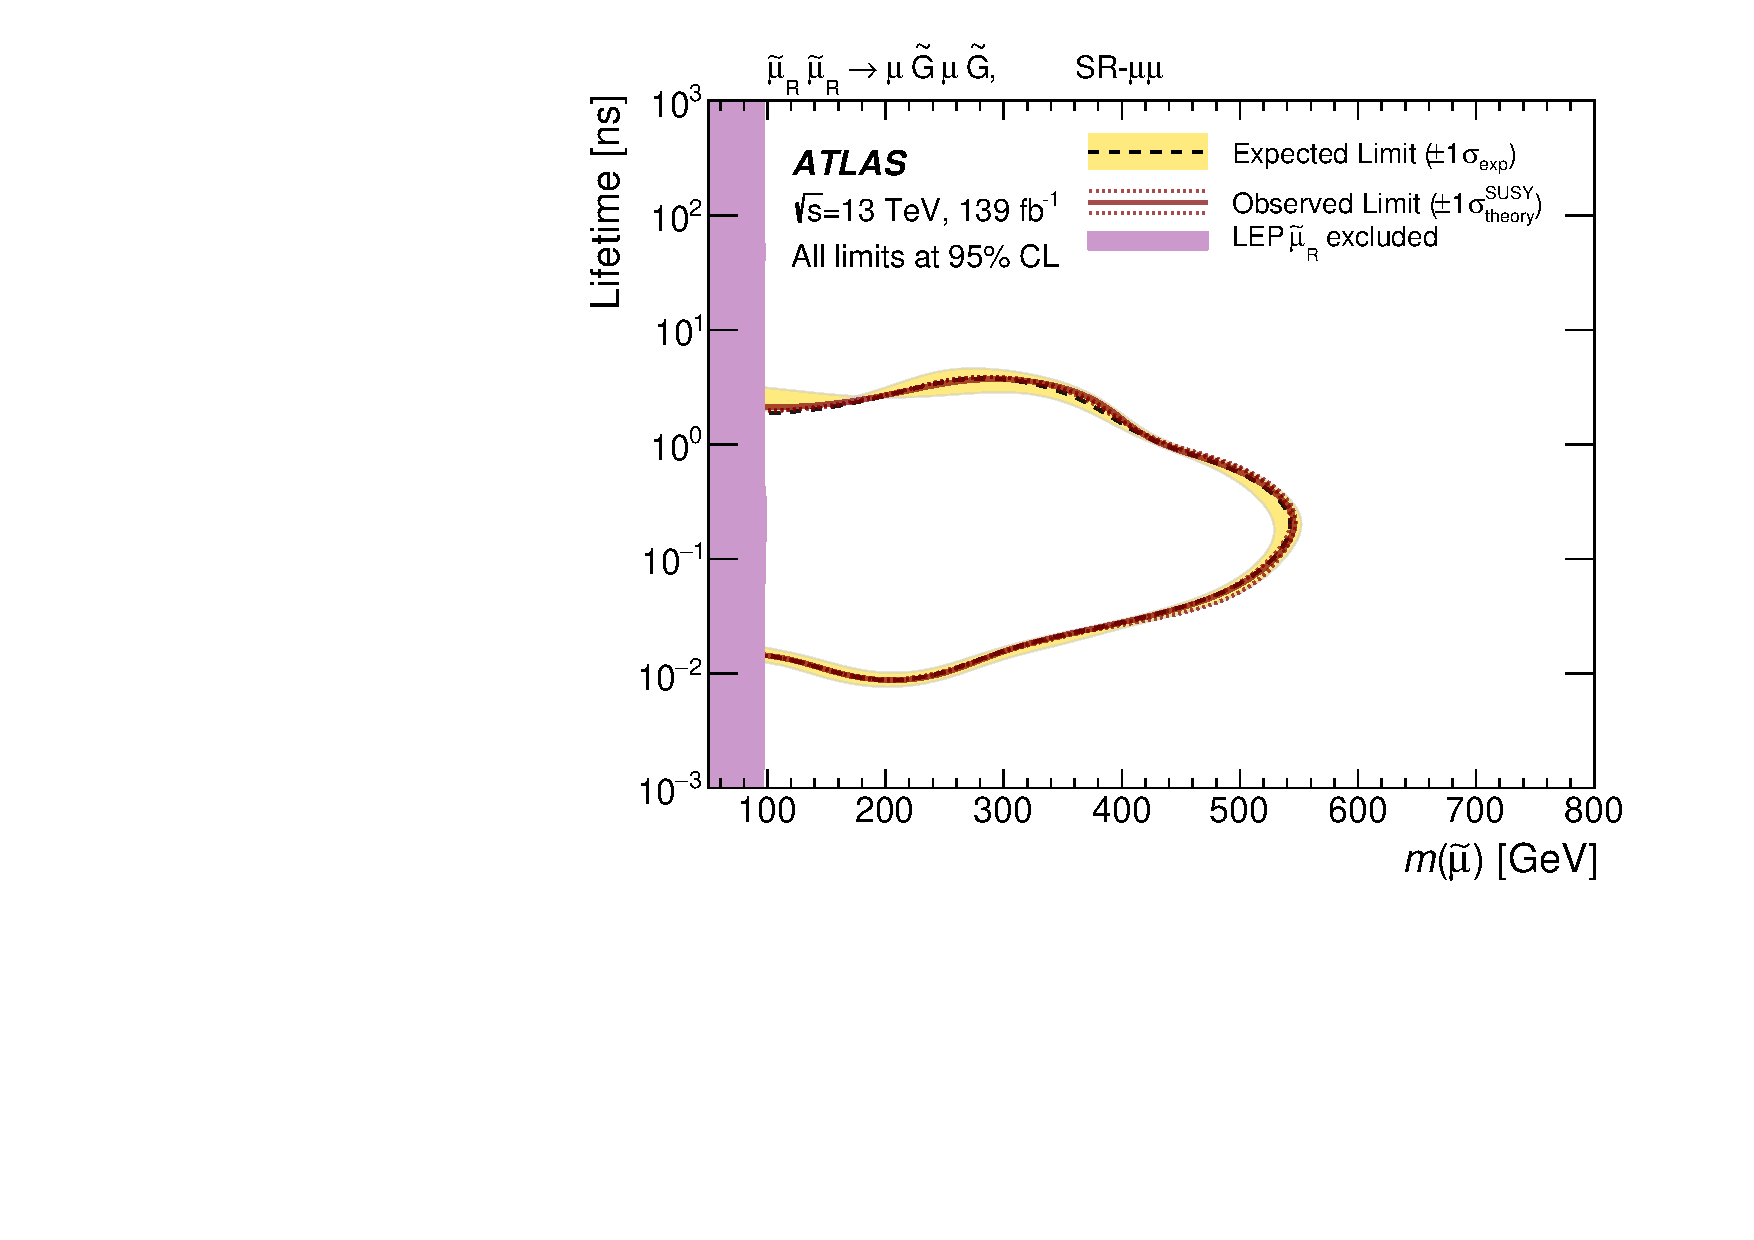
\includegraphics[width=0.45\textwidth]{figures/limits/SRmm_Slepright.pdf}
        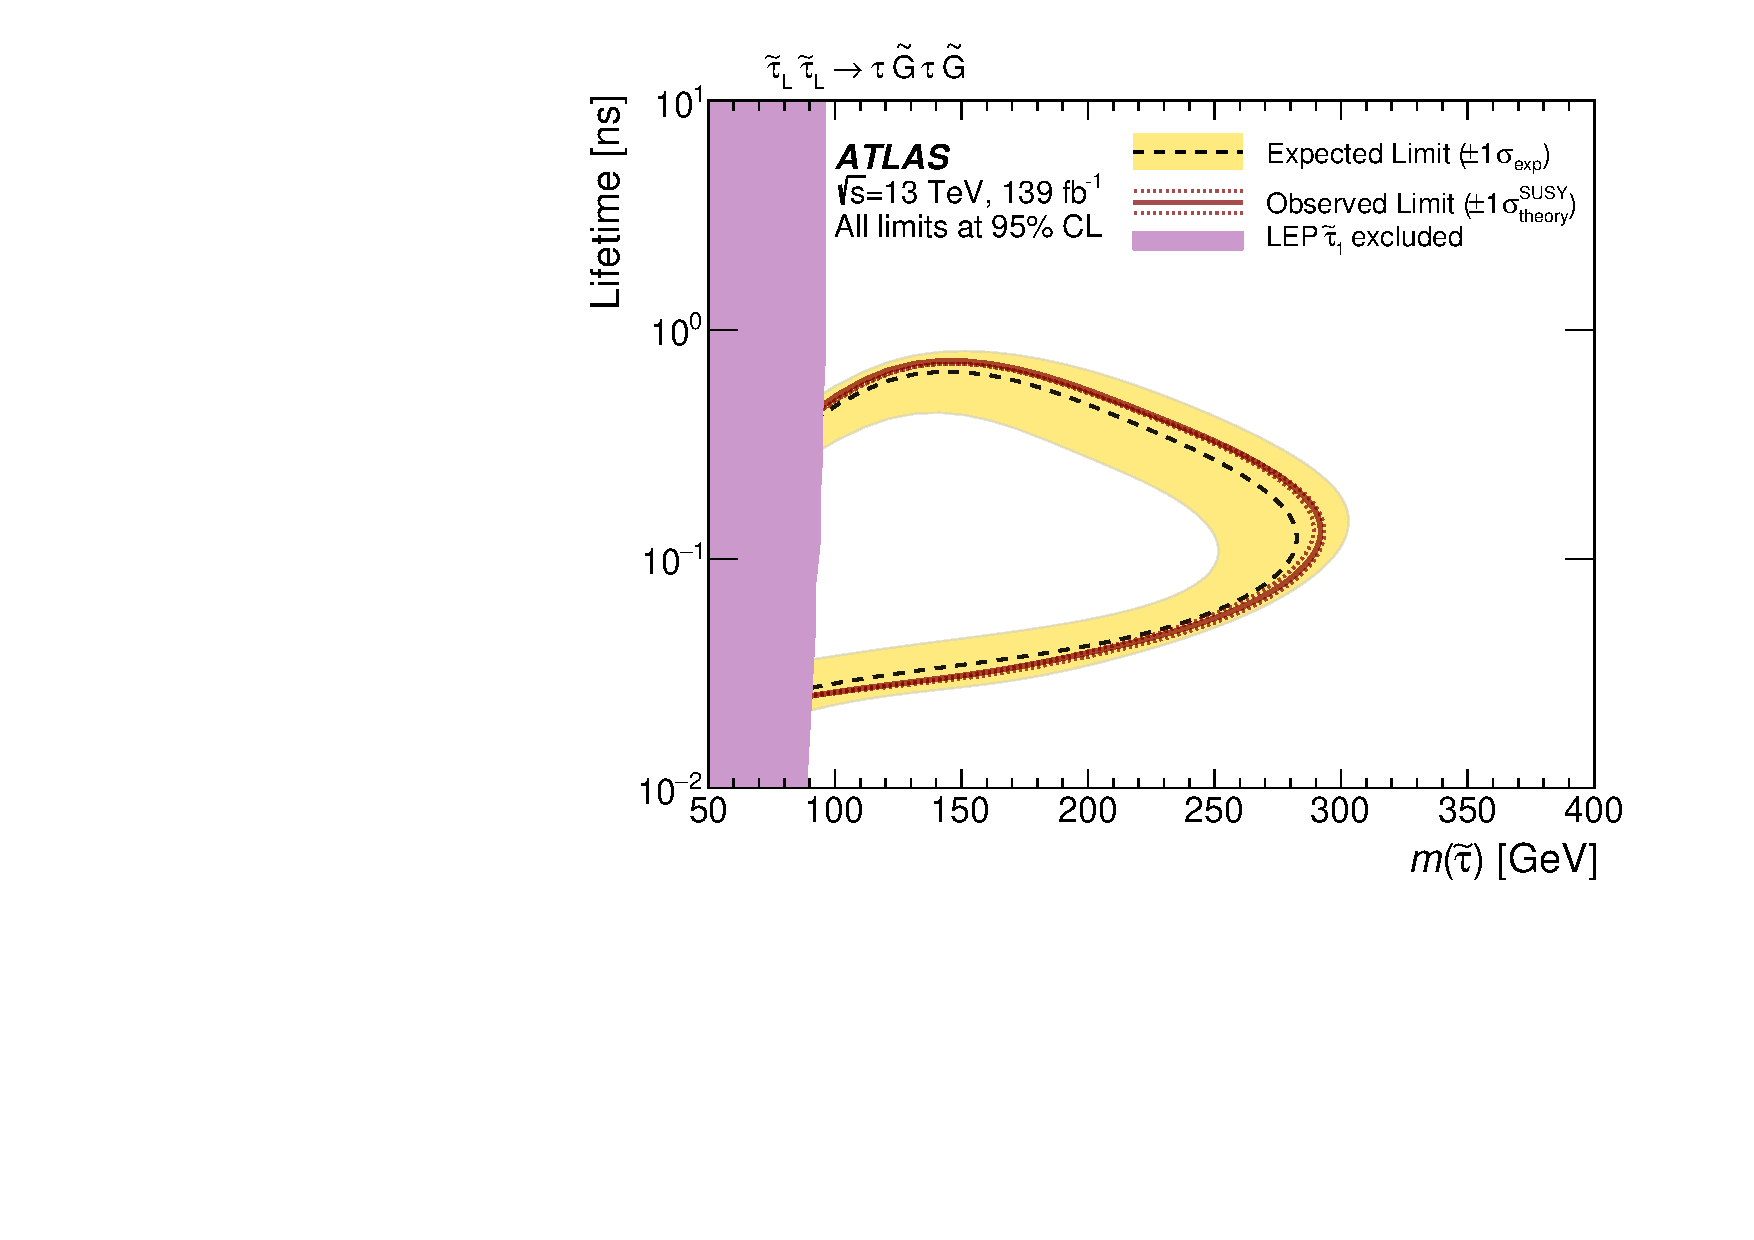
\includegraphics[width=0.45\textwidth]{figures/limits/Stauleft.pdf}
    \caption{Limits on \slep separated by their chirality with the \ac{LEP} limit shown in pink. In order from top to bottom, left to right: $\selec_{L}$, $\selec_{R}$, $\smu_{L}$, $\smu_{R}$, left-handed $\stau_{1}$. This result does not have significant sensitivity to right-handed $\stau_{2}$.}
    \label{fig:lep_comp}
\end{figure}

\FloatBarrier

\section{Model-Indpendent Limits}
Additionally, model independent limits are set on generic new physics processes in the \acp{SR}. These limits are based on the visible cross-section of new physics ($\langle \epsilon \sigma^{95}_{\text{obs}} \rangle$) and the observed ($S^{95}_{\text{obs}}$) and expected ($S^{95}_{\text{exp}}$) number of signal events that would be measured. Visible \ac{BSM} cross sections above 0.02 fb are excluded in each \ac{SR} These values are shown in \autoref{table.results.exclxsec.pval.upperlimit.SR}

\begin{table}[hbt]
\centering
\begin{tabular*}{\textwidth}{@{\extracolsep{\fill}}lccccccc}
\noalign{\smallskip}\noalign{\smallskip}
{ Signal channel} & $\langle\epsilon{ \sigma}\rangle_\text{obs}^{95}$[fb]  &  $S_\text{ obs}^{95}$  & $S_\text{ exp}^{95}$  
\\
\noalign{\smallskip}\hline\noalign{\smallskip}
%%
 SR-$ee$   & $0.02$ &  $3.0$ & $ 3.0$   \\%                                                                                 
 SR-$\mu\mu$   &$0.02$ &  $3.0$ & $ 3.0$  \\%                                                                               
SR-$e\mu$   &$0.02$ &  $2.7$ & $ 3.0$  \\%
\noalign{\smallskip}\hline\noalign{\smallskip}
\end{tabular*}
\caption[Breakdown of upper limits.]{
Left to right: 95\% CL upper limits on the visible cross section
($\langle\epsilon\sigma\rangle_\text{ obs}^{95}$) and on the number of
signal events ($S_\text{ obs}^{95}$ ).  The third column
($S_\text{ exp}^{95}$) shows the 95\% CL upper limit on the number of
signal events, given the expected number of background events. The last column shows the p-value of the no-signal hypothesis.
\label{table.results.exclxsec.pval.upperlimit.SR}}
\end{table}